\documentclass{xjtureport}
% =============================================
% Part 0 Edit the info
% =============================================

\major{计算机001班}
\name{曾锦程}
\title{SDN实验报告}
\stuid{2203613040}
\college{计算机学院}
\date{\zhtoday}
\lab{}
\course{软件定义网络}
\instructor{张鹏}
\grades{}
\expname{Lab4 VeriFlow网络验证}
\exptype{设计实验}
\partner{}

\begin{document}
% =============================================
% Part 1 Header
% =============================================
\makecover
\makeheader
\tableofcontents
\newpage
% =============================================
% Part 2 Main document
% =============================================

\section{实验目的}
1.理解网络故障的普遍性\par 
2.熟悉网络验证工具 \textbf{veriflow} 的原理 \par 
3.掌握 \textbf{veriflow} 的故障检测方法 \par 
\section{问题背景}
\begin{figure}[H]
	\centering
	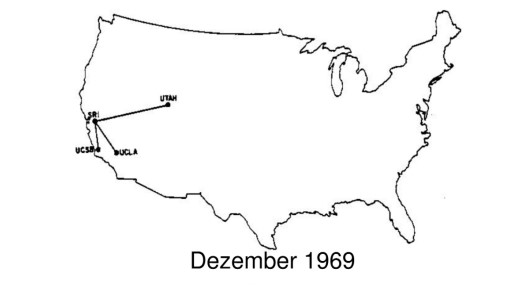
\includegraphics[width=0.9\linewidth]{1.jpg}
	\caption{TOPO}
\end{figure}
TINKER 处建立了一个流量分析中心,为了保证 UTAH 和 ILLINOIS 之间的流量可以在 TINKER 进行分
析,你下发了图中的红色路径。你的同事Bob接到了另外一个需求,要求建立从 SDC 到 MIT 跳数最少的
路径,即图中的绿色路径。不同的路径需求来自不同的用户,没有经过协调,产生了一个转发环路。请
你运行 VeriFlow 工具,对上述两条转发路径进行检查,完成以下实验内容。
\section{基本实验理论}
以下介绍VeriFlow的基本原理:
\subsection{生成等价类(Generate equivalence classes)}
在Veriflow中,生成等价类是指将网络中的流量路径划分为不同的等价类。等价类是具有相同属性或行为的流量路径的集合。Veriflow根据网络的不同属性(例如源IP地址、目标IP地址、端口号、协议类型等)将流量路径分组为等价类。这样的划分可以将验证问题的规模和复杂性降低到可管理的程度。通过生成等价类,Veriflow可以在每个等价类中独立地进行验证分析,以检测潜在的网络配置错误和安全漏洞。
\subsection{生成转发图(Generate forwarding graphs):}
在Veriflow中,生成转发图是指根据网络的拓扑结构和设备配置生成数据包的预期转发路径。Veriflow使用数据收集阶段获取的网络拓扑信息、路由表和转发规则等,构建网络的转发图。这个图描述了数据包从源设备到目标设备的预期路径,包括中间设备和链路。通过生成转发图,Veriflow能够准确模拟和分析数据包在网络中的转发行为。
\subsection{运行查询(Run queries)}
运行查询是Veriflow的最后一步,用于执行特定的验证查询或分析请求。在此步骤中,Veriflow使用生成的等价类和转发图来回答用户的查询。用户可以提出不同类型的查询,例如验证两个主机之间的通信路径是否满足特定的安全策略,检测网络中的冗余路径,识别访问控制规则的冲突等。Veriflow运行查询并分析等价类和转发图,以确定网络是否符合预期的行为和安全策略。
\section{基础实验部分}
\subsection{实验要求}
请运行VeriFlow工具,对上述两条转发路径进行检查,完成下述基础实验\par
1. 输出每次影响EC的数量 \par
2. 打印出环路路径的信息 \par 
3. 进一步打印出环路对应的EC的相关信息 \par 
4. 分析原始代码与补丁代码的区别,思考为何需要添加补丁 \par
\subsection{实验原理}
\subsubsection{实验拓扑图}
为了更好的理解环路形成过程,这里筛选出必要部分的拓扑图,方便观察。
\begin{figure}[H]
	\centering
	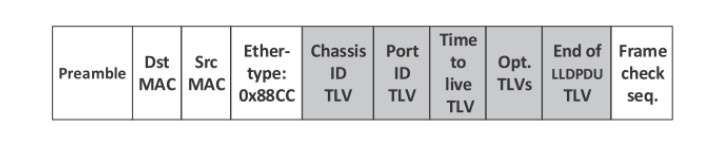
\includegraphics[width=0.9\linewidth]{2.jpg}
	\caption{必要拓扑图}
\end{figure}
\subsubsection{环路形成过程}
在形成环路过程中,有以下几个过程:\par 
(I)先在Mininet里面SDC ping MIT\par 
\quad \quad 在ping的过程中下发如下图流表:
\begin{figure}[H]
	\centering
	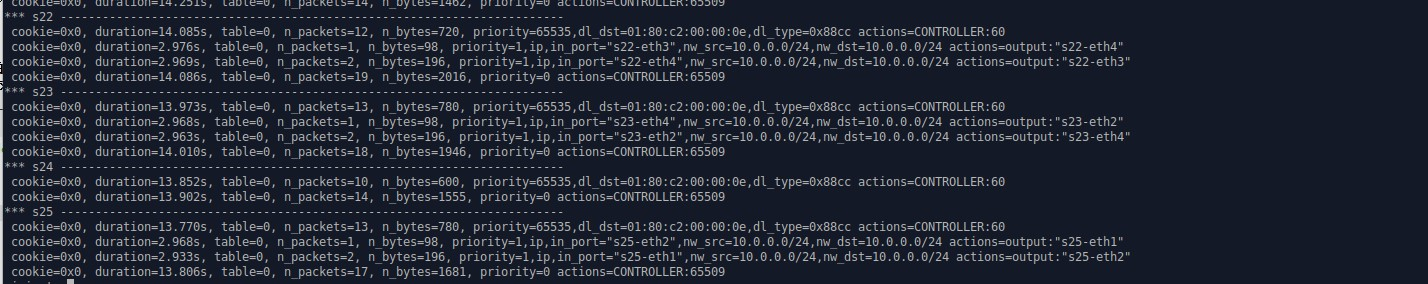
\includegraphics[width=0.9\linewidth]{3.jpg}
	\caption{下发流表}
\end{figure}
\quad \quad 在ping的过程中下发如下图路径:
\begin{figure}[H]
	\centering
	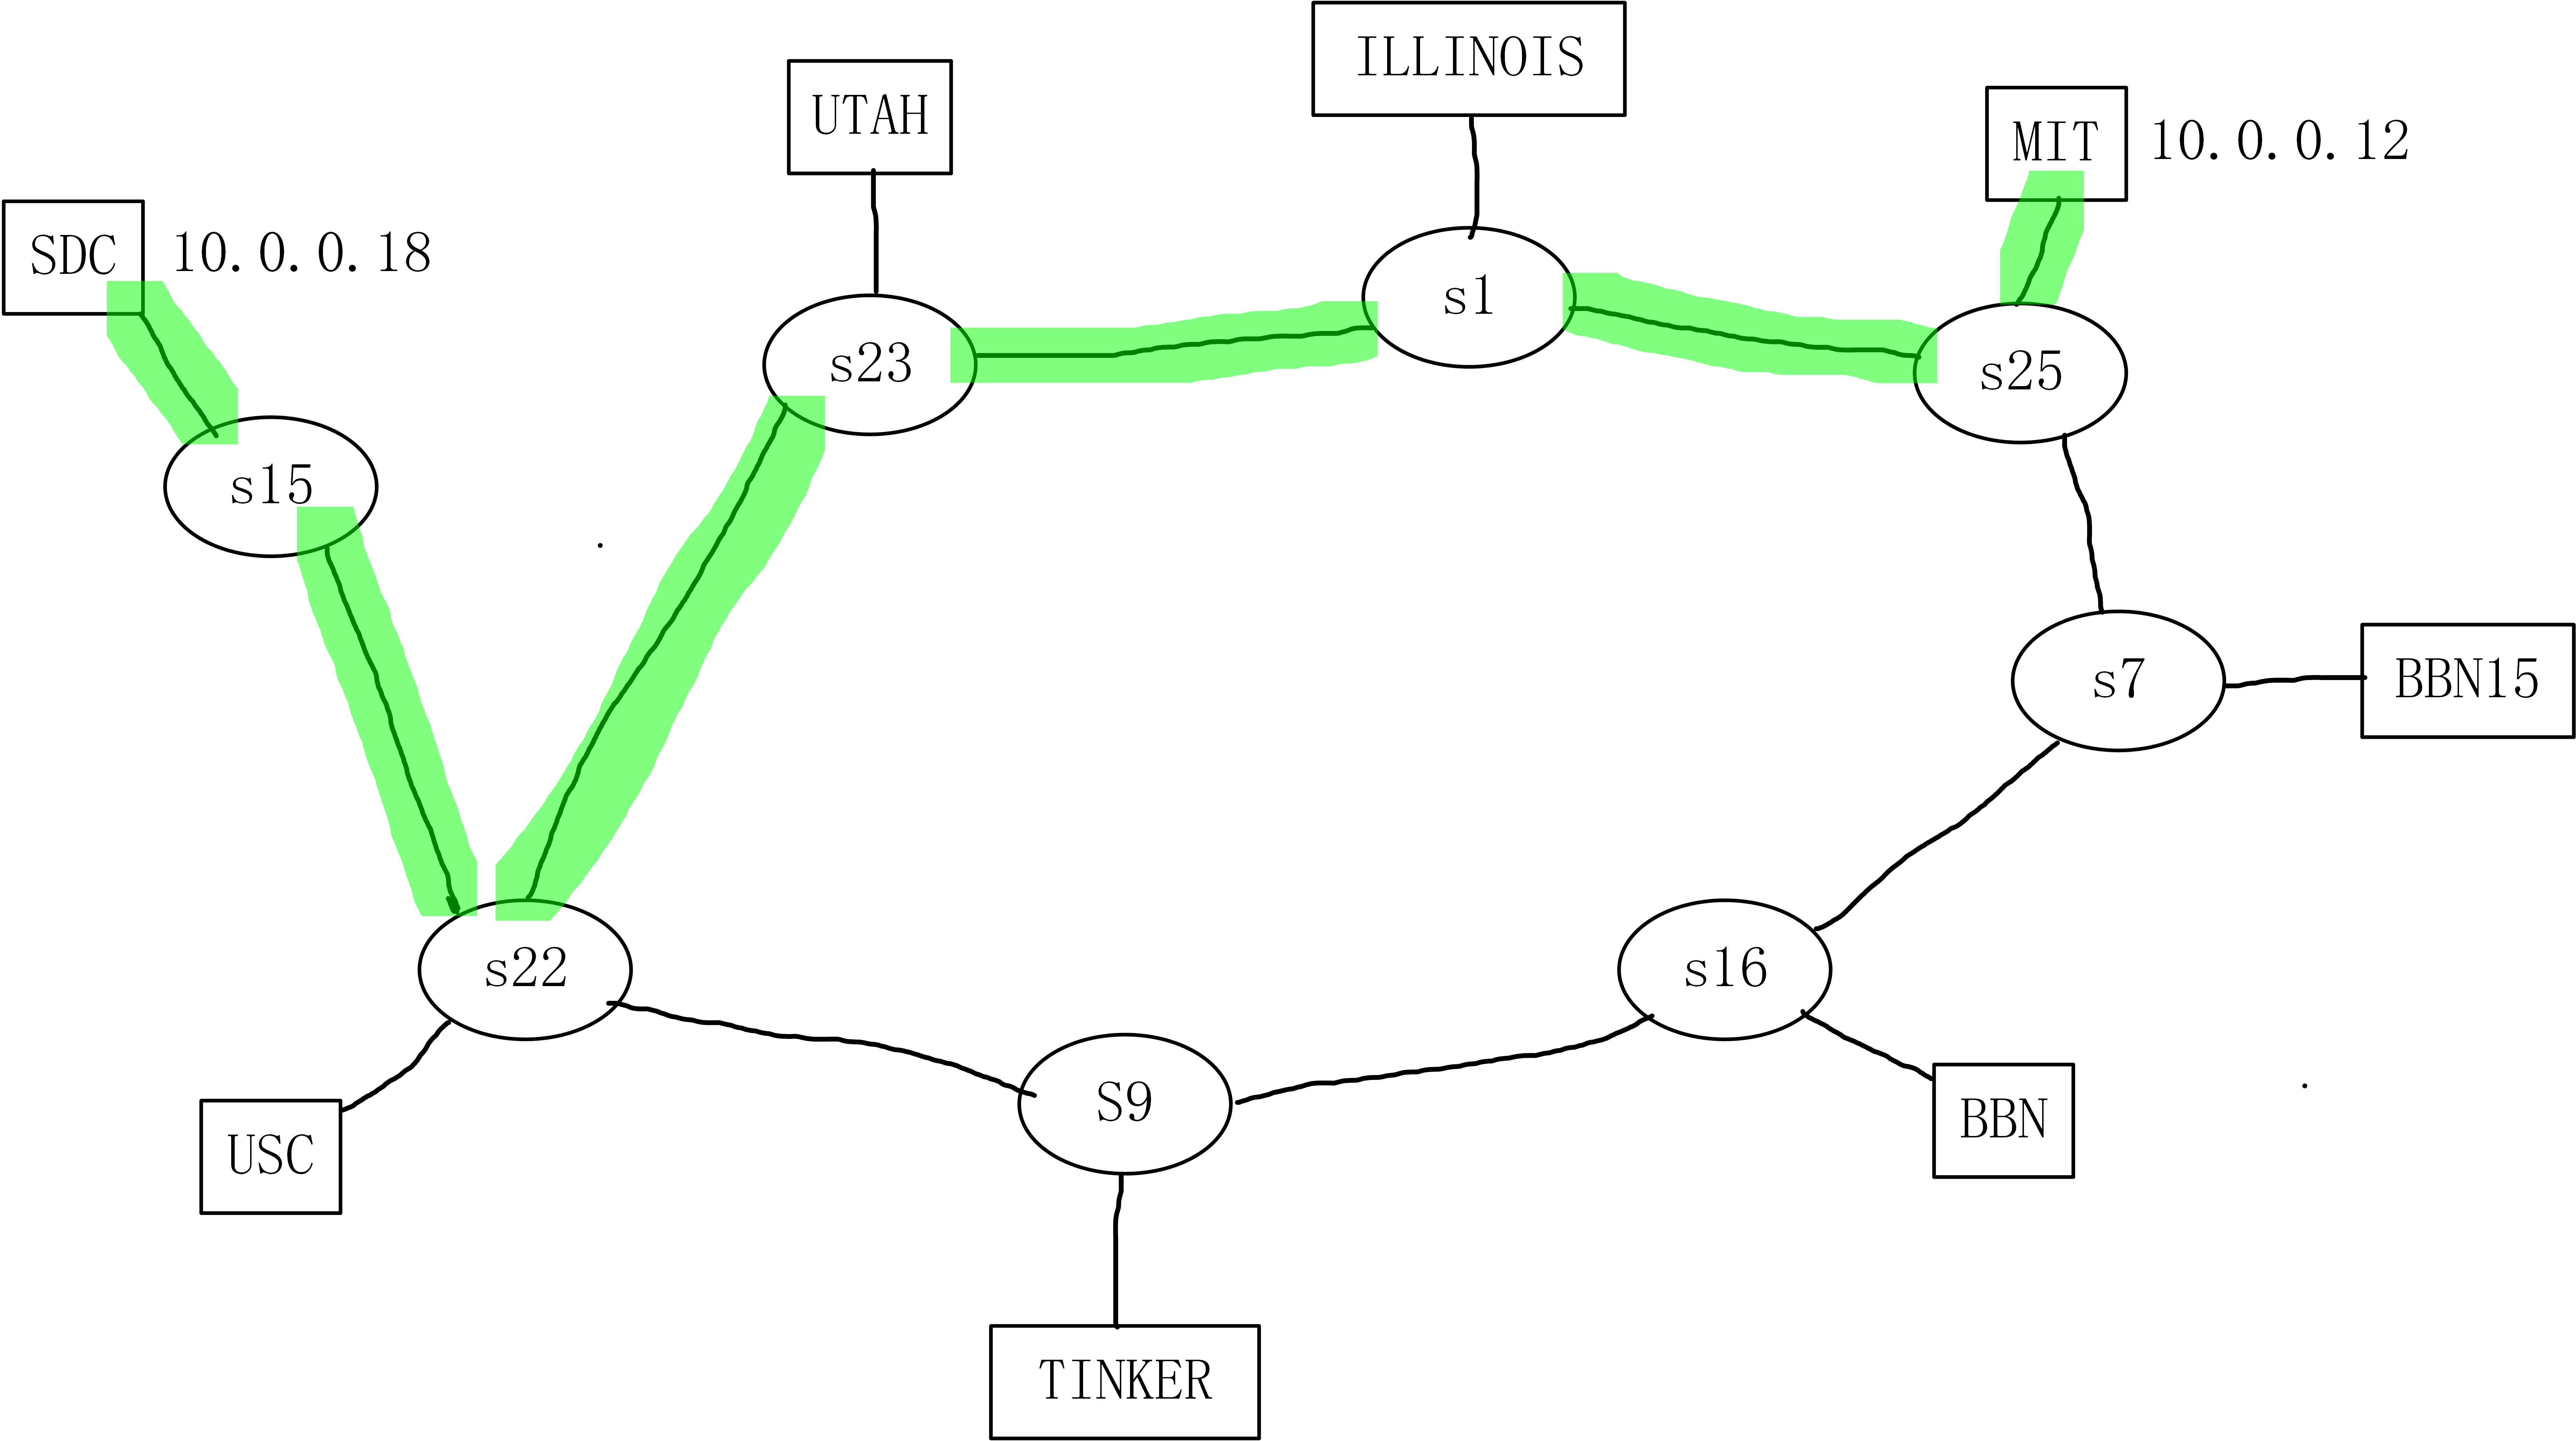
\includegraphics[width=0.9\linewidth]{4.jpg}
	\caption{下发路径}
\end{figure}
(II)ping通后,运行waypoint\_path.py\par 
\quad \quad 下发如下图流表:
\begin{figure}[H]
	\centering
	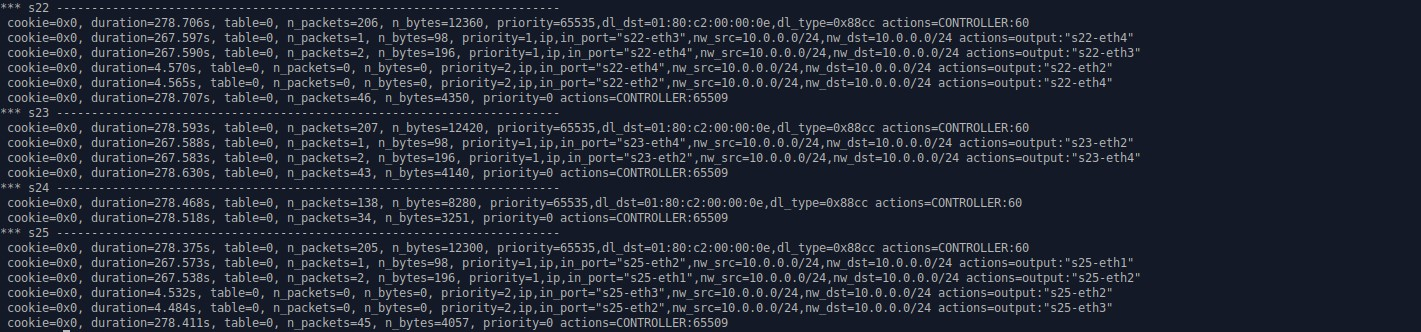
\includegraphics[width=0.9\linewidth]{5.jpg}
	\caption{下发路径}
\end{figure}
\quad \quad 下发如下图路径:
\begin{figure}[H]
	\centering
	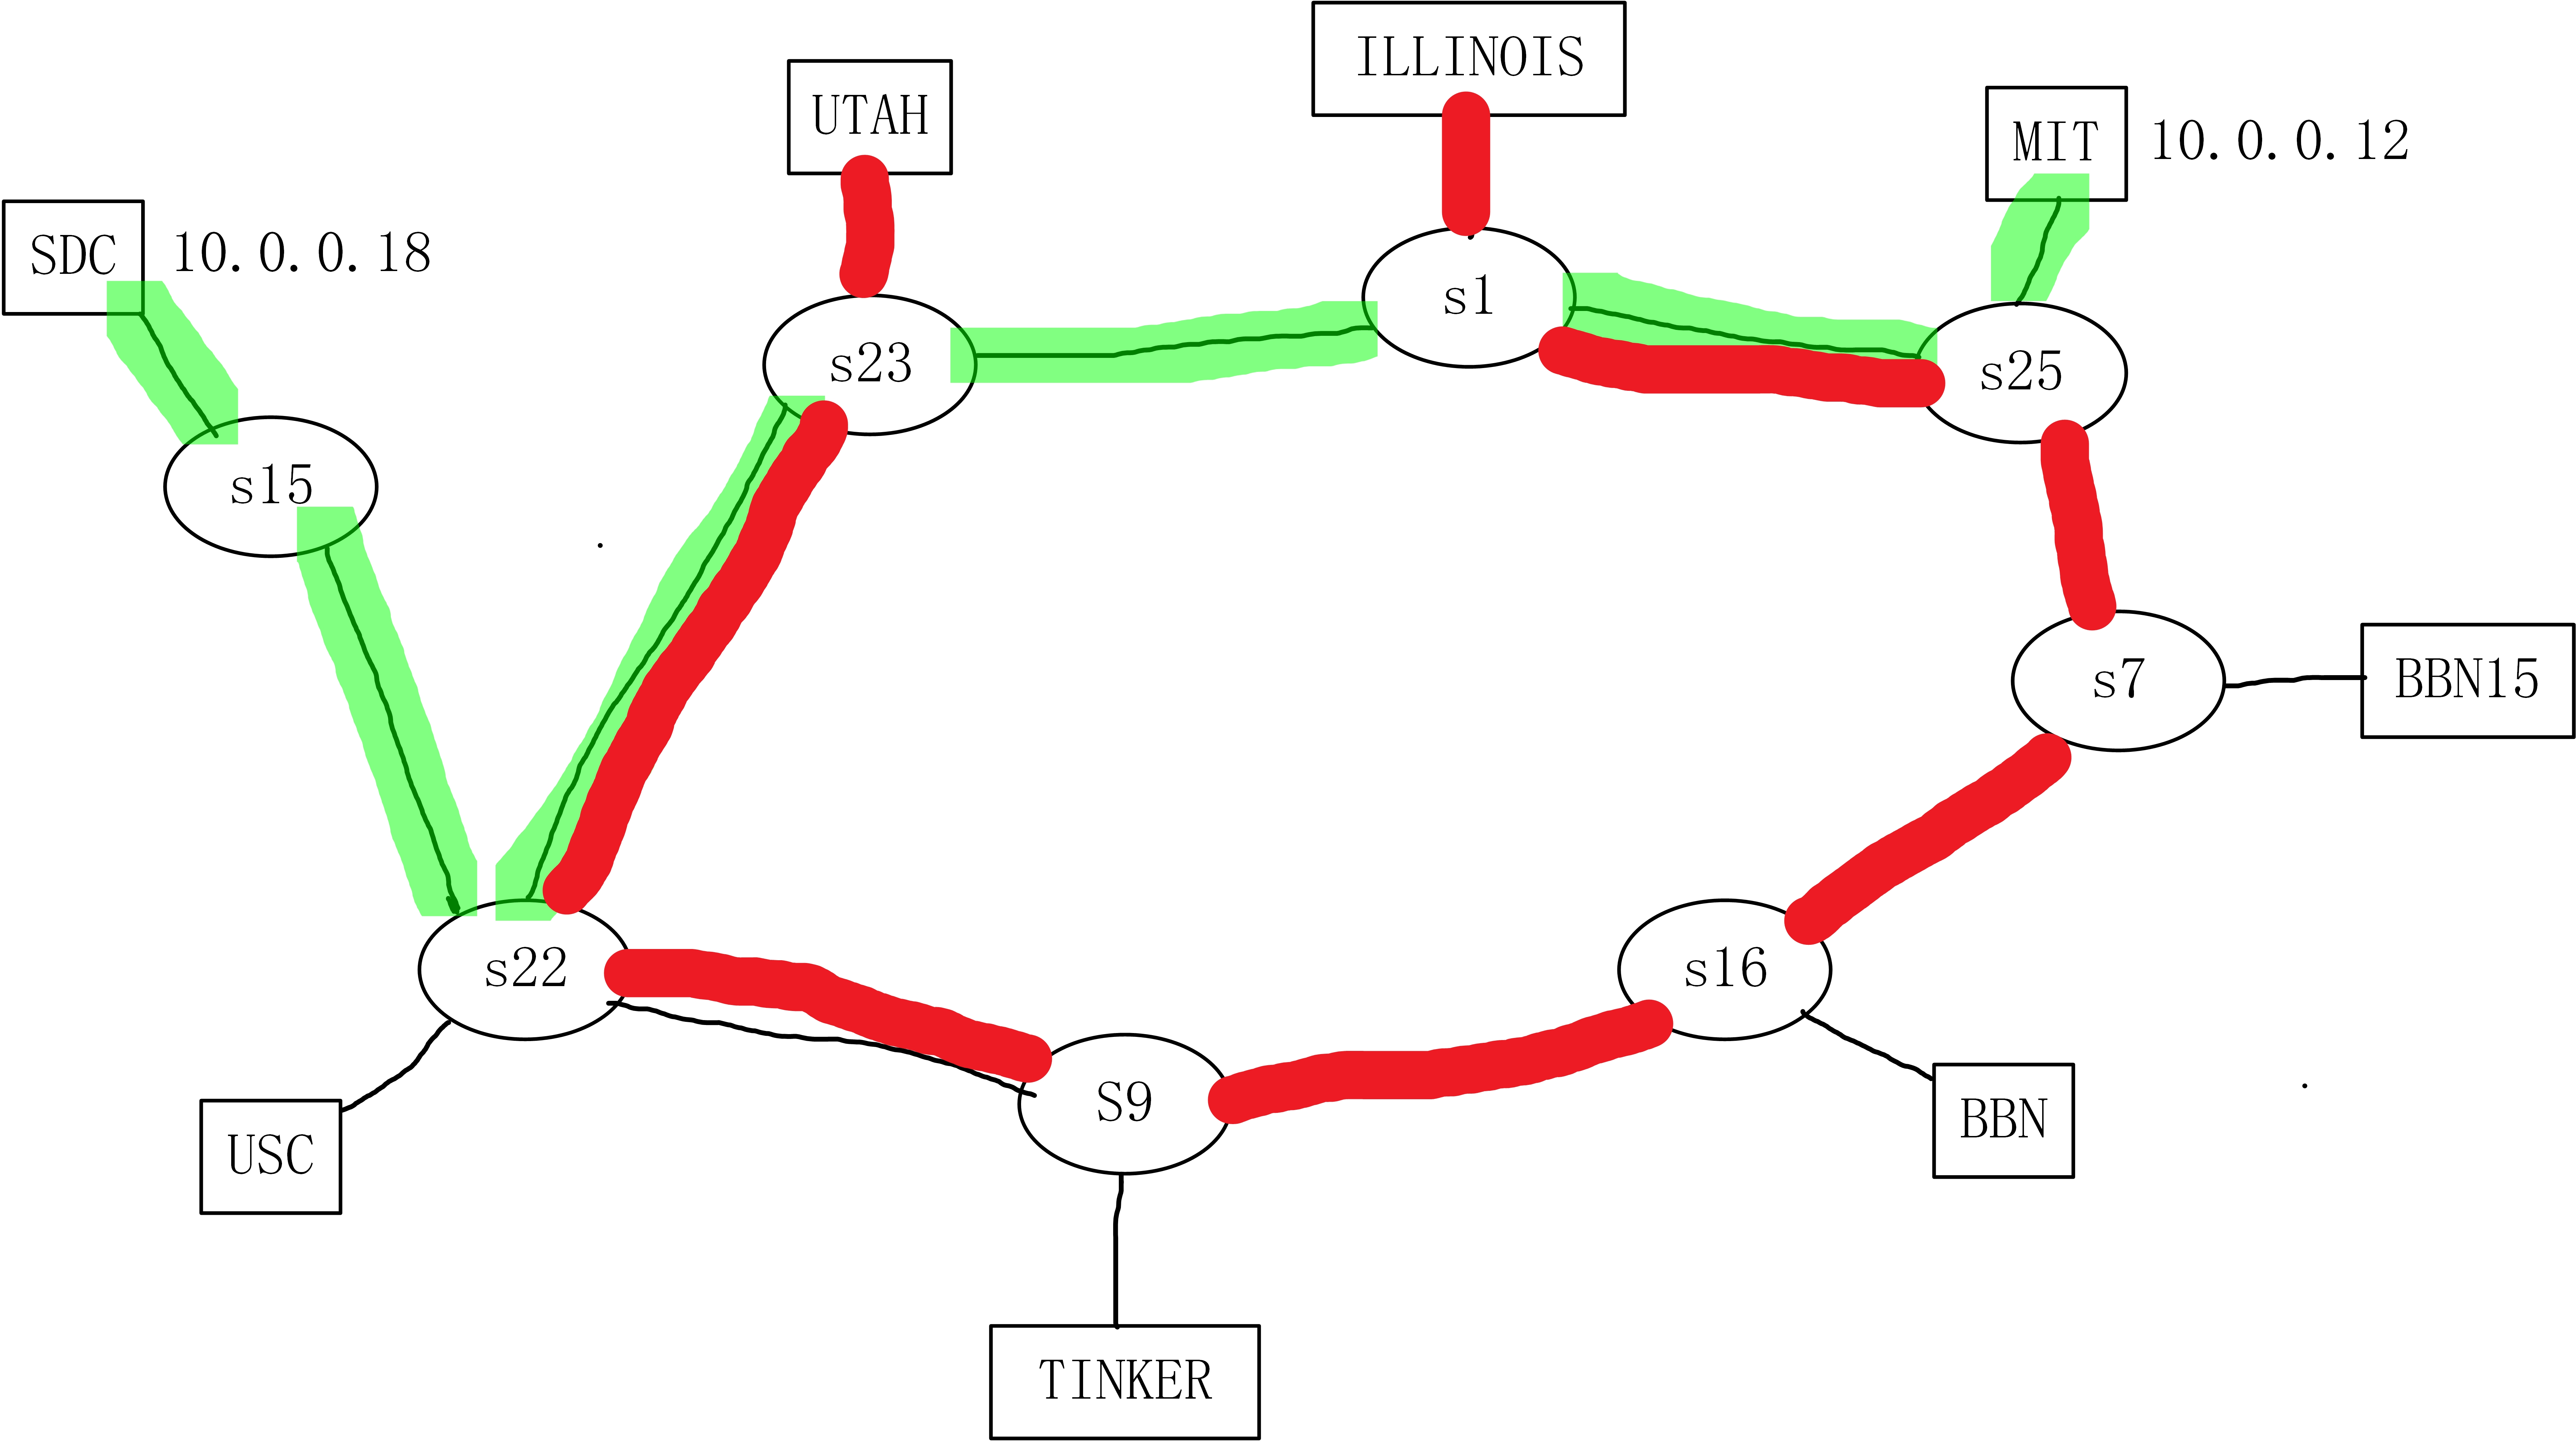
\includegraphics[width=0.9\linewidth]{6.jpg}
	\caption{下发路径}
\end{figure}
(III)形成环路\par 
\begin{figure}[H]
	\centering
	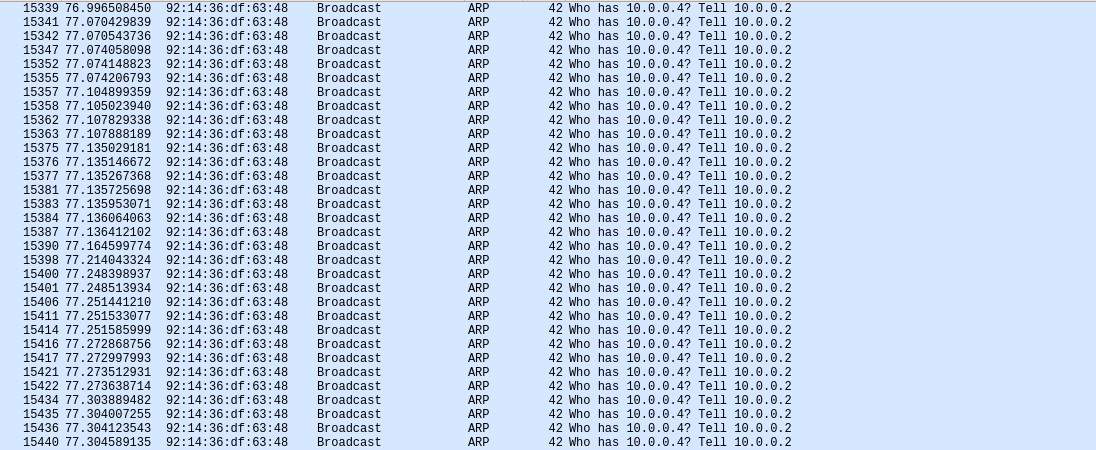
\includegraphics[width=0.9\linewidth]{7.jpg}
	\caption{环路路径}
\end{figure}
关键在于s22和s25的流表改变,导致SDC到MIT的数据包转发错误,形成了如上图所示蓝色和紫色两条环路。
\subsection{输出每次影响EC的数量}
对VeriFlow类中的\texttt{verifyRule()}函数进行如下修改,将等价类的输出放到fp,即log\_file.txt文件中
\begin{lstlisting}[language=c++]
bool VeriFlow::verifyRule(){
	...
	ecCount = vFinalPacketClasses.size();
	if(ecCount == 0)
	{
		fprintf(stderr, "[VeriFlow::verifyRule] Error in rule: %s\n", rule.toString().c_str());
		fprintf(stderr, "[VeriFlow::verifyRule] Error: (ecCount = vFinalPacketClasses.size() = 0). Terminating process.\n");
		//fprintf(fp, "[VeriFlow::verifyRule] Error: (ecCount = vFinalPacketClasses.size() = 0). Terminating process.\n");
		exit(1);
	}
	else
	{
		fprintf(stdout, "\n");
		fprintf(stdout, "[VeriFlow::verifyRule] ecCount: %lu\n", ecCount);
		fprintf(fp, "[VeriFlow::verifyRule] ecCount: %lu\n", ecCount);
	}
	...
}
\end{lstlisting}
\subsection{打印出环路路径的信息}
对VeriFlow类中的\texttt{traverseForwardingGraph()}函数进行如下修改,引入与visited类似的vector的 loop\_path,与visited插入相同,为递归式插入,但是有序,在检测出网络系统中存在环路时,在loop\_path找到起始点后按序输出所有路径。
\begin{lstlisting}[language=c++]
bool VeriFlow::traverseForwardingGraph(const EquivalenceClass& packetClass, ForwardingGraph* graph, const string& currentLocation, const string& lastHop, unordered_set< string > visited, FILE* fp, vector<string> loop_path){
	...
	if(visited.find(currentLocation) != visited.end())
	{
		// Found a loop.
		fprintf(fp, "\n");
		fprintf(fp, "[VeriFlow::traverseForwardingGraph] Found a LOOP for the following packet class at node %s.\n", currentLocation.c_str());
		fprintf(fp, "[VeriFlow::traverseForwardingGraph] PacketClass: %s\n", packetClass.toString().c_str());
		fprintf(fp, "[VeriFlow::traverseForwardingGraph] Loop path is:\n");
		bool judge = false;
		for(unsigned int i=0;i<loop_path.size()-1;i++){
			if(loop_path[i]==currentLocation){
				judge=true;
			}
			if(judge){
				fprintf(fp, "%s --> ", loop_path[i].c_str());
			}
		}
		fprintf(fp, "%s\n", currentLocation.c_str());
		for(unsigned int i = 0; i < faults.size(); i++) {
			if (packetClass.subsumes(faults[i])) {
				faults.erase(faults.begin() + i);
				i--;
			}
		}
		faults.push_back(packetClass);
		
		return false;
	}
	visited.insert(currentLocation);
	loop_path.push_back(currentLocation);
	...
}
\end{lstlisting}
\subsection{进一步打印出环路对应的EC的相关信息}
在EquivalenceClass类中修改函数\texttt{toString()}函数,将原来的输出,改成输出标准TCP/IP五元组,即使(IP源地址,IP目的地址,网络层协议类型,传输层源端口号,传输层目的端口号)。
\begin{lstlisting}[language=c++]
	string EquivalenceClass::toString() const
	{
		char buffer[1024]={'\0'};
		string retVal = buffer;
		sprintf(buffer, "nw_src(%s-%s), nw_dst(%s-%s)",
		::getIpValueAsString(this->lowerBound[NW_SRC]).c_str(),
		::getIpValueAsString(this->upperBound[NW_SRC]).c_str(),
		::getIpValueAsString(this->lowerBound[NW_DST]).c_str(),
		::getIpValueAsString(this->upperBound[NW_DST]).c_str());
		retVal += buffer;
		retVal += ", ";
		sprintf(buffer, "nw_proto(%lu-%lu), tp_src(%lu-%lu), tp_dst(%lu-%lu)",
		this->lowerBound [NW_PROTO],
		this->upperBound [NW_PROTO],
		this->lowerBound [TP_SRC],
		this->upperBound [TP_SRC],
		this->lowerBound [TP_DST],
		this->upperBound [TP_DST]);
		retVal += buffer;		
		return retVal;
	}
\end{lstlisting}	
\subsection{最终输出结果}
可以通过观察VeriFlow的结果与上述分析相一致,只有下发在s22和s25的两条流表规则对环路造成了影响。
\begin{figure}[H]
	\centering
	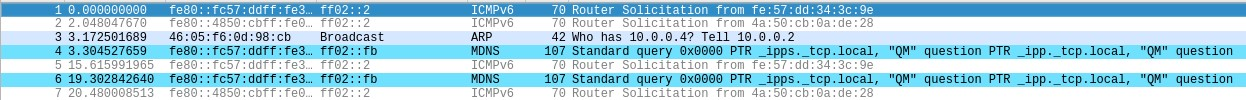
\includegraphics[width=0.9\linewidth]{8.jpg}
	\caption{最终结果}
\end{figure}
\subsection{分析原始代码与补丁代码的区别,思考为何需要添加补丁}
(1)改动一:匹配域in\_port的增加\par 
第一个改动主要是流表规则中添加in\_port属性,这实际上是合理的,流表规则实际上是需要in\_port属性的,不同的入端口可能导致不一样的转发规则。\par
如图9,主要是在处理流表的过程中,添加了in\_port属性的处理修改。
\begin{figure}[H]
	\centering
	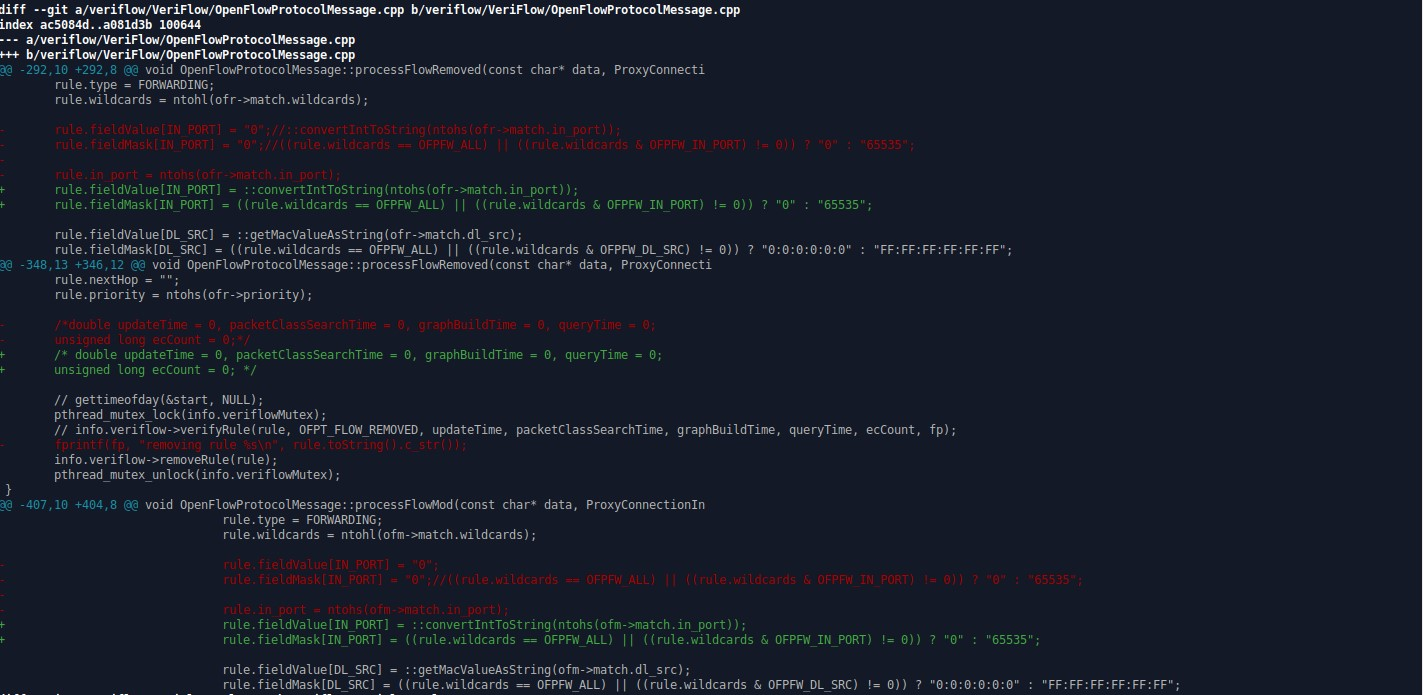
\includegraphics[width=0.9\linewidth]{9.jpg}
	\caption{VeriFlow类的改动}
\end{figure}
如图10,主要是在Rule类中,即流表规则,加入了in\_port匹配域,判等函数,拷贝构造函数,转字符串函数等等,能够更精确地区分不同流表规则,这是合理且必要的。
\begin{figure}[H]
	\centering
	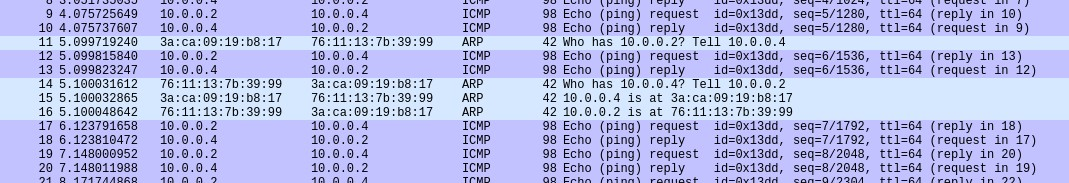
\includegraphics[width=0.9\linewidth]{12.jpg}
	\caption{Rule类的改动}
\end{figure}
(2)改动二:网络黑洞判定补充\par 
原代码判定网络黑洞方法:\par
(i)当前节点,没有流表指向输出链路\par 
(ii)图中不存在当前节点\par   
\begin{figure}[H]
	\centering
	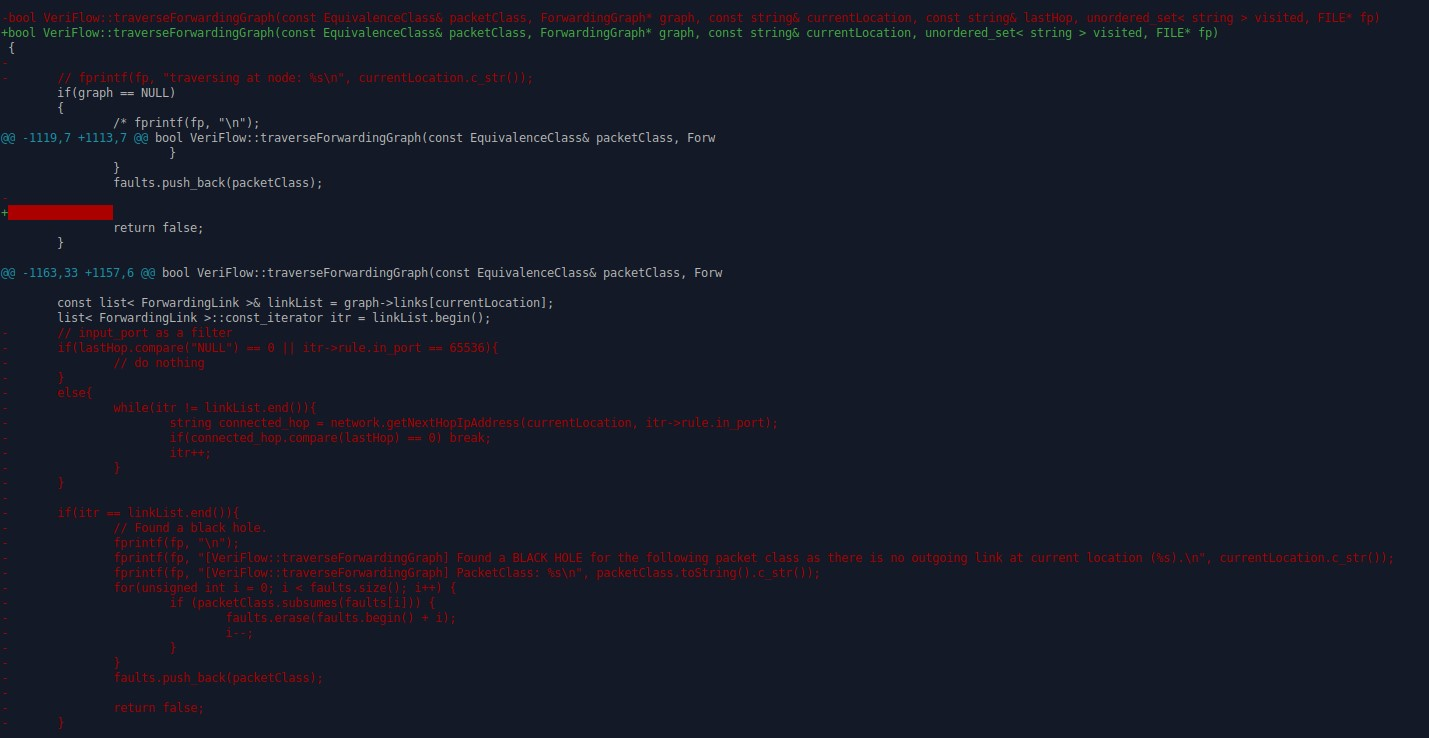
\includegraphics[width=0.9\linewidth]{11.jpg}
	\caption{新加黑洞判定规则}
\end{figure}
补丁代码增加判定方法:\par
(i)改节点的上一跳在图中不存在\par
这一判定方法实际上是加入了in\_port字段而导致的,如果该规则的流表项的in\_port不为65536(即缺省值)且上一跳不为空(即不为初始节点),则需要判断上一条的存在性,确保in\_port字段的规则验证是合理有效的。 \par
比如下发的流表固定了端口,in\_port连接了交换机A,但是下发的规则可能走了其他路径通过连接该交换机的交换机B,也传输数据包到该交换机,如果是原代码则会不管,顺利地下发该规则,但是这是明显不合理的,来自交换机B的数据包实际不可能走该流表,这样验证就导致了错误,这样的验证工具是不完备的。\par
(3)改动三:下一跳转发优化\par
补丁中,in\_port的加入实际上还优化了下一跳的寻路,使得Run Query的过程中,不会形成从交换机A到B,又从交换机B到A的循环,这样的情况在未打补丁的代码中是有情况会出现的,而加入了in\_port的限制则不会,如果流表具有in\_port部分,是不会启动上一跳链接的查询的。
 \begin{figure}[H]
	\centering
	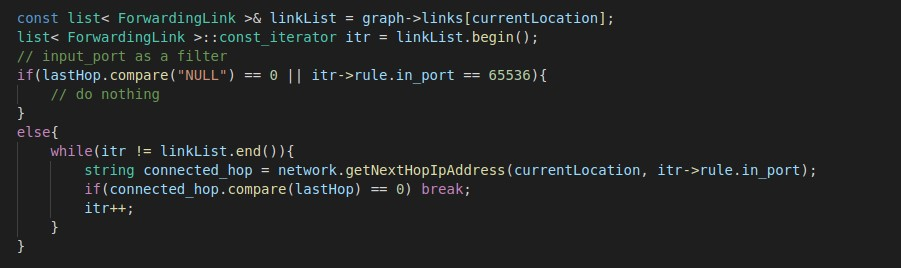
\includegraphics[width=0.9\linewidth]{26.jpg}
	\caption{下一跳转发优化}
 \end{figure}
 \begin{figure}[H]
 	\centering
 	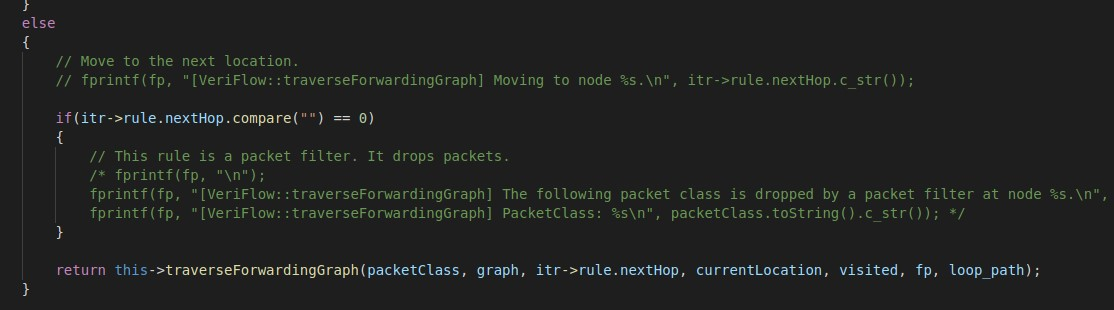
\includegraphics[width=0.9\linewidth]{25.jpg}
 	\caption{下一跳转发优化}
 \end{figure}
\section{拓展实验部分}
\subsection{实验要求}
1. 若修改 waypoint\_path.py 代码中被添加规则的优先级字段,VeriFlow的检测结果会出错,试描述错误是什么,并解释出错的原因\par
2. 在VeriFlow支持的14个域中,挑选多个域(不少于5个)进行验证,输出并分析结果\par
\subsection{修改优先级出错原因}
对比设置两种优先级的输出结果:\par 
(1)实际网络情况:两种方法都会造成环路,因为对相同优先级别的匹配域相同流表来说,交换机会用新流表覆盖旧流表,如下图所示\par
\begin{figure}[H]
	\centering
	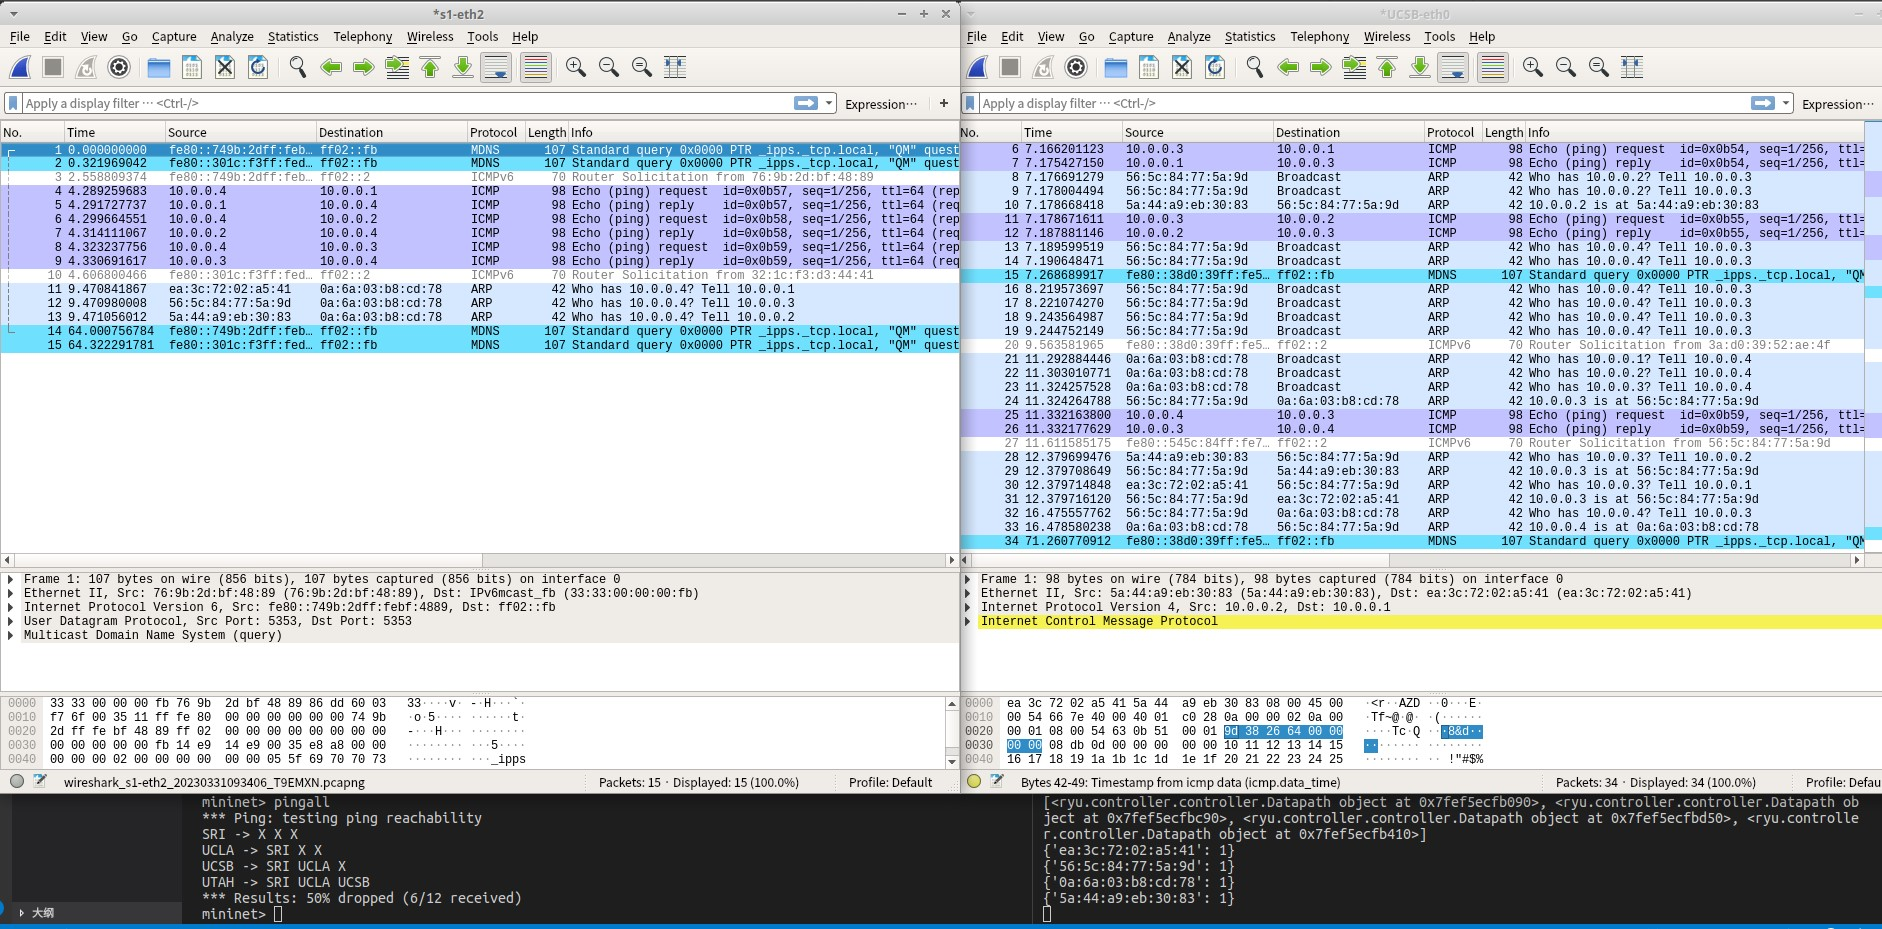
\includegraphics[width=0.9\linewidth]{13.jpg}
	\caption{流表覆盖现象}
\end{figure}
(2)VeriFlow网络验证情况:不同优先级会造成检测出环路,而相同优先级不会检测出环路\par
可以看出最下面的流表,直接不输出等价类和验证结果,这就是判定相同流表,而不添加导致的。\par
\begin{figure}[H]
	\centering
	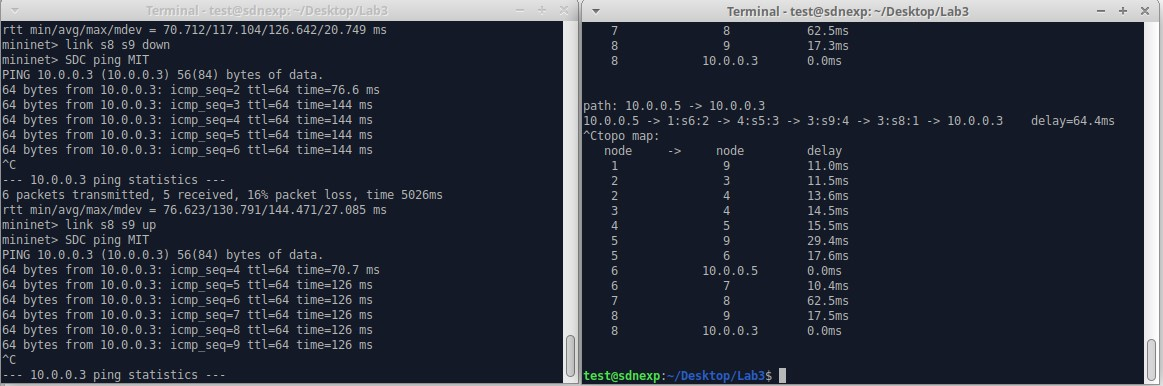
\includegraphics[width=0.9\linewidth]{14.jpg}
	\caption{验证情况区别}
\end{figure}
主要的问题出现在如下代码中,对于已经存在的规则,\texttt{addRule()}函数会进行抛弃。
\begin{lstlisting}[language=c++]
bool VeriFlow::addRule(const Rule& rule)
{
	...
				unordered_set< Rule, KHash< Rule >, KEqual< Rule > >::const_iterator itr;
				itr = leaf->ruleSet->find(rule);
				if(itr != leaf->ruleSet->end()) // Rule already exists.
				{
					fprintf(stderr, "This Rule is already exists.");
					return false;
				}
			}
			
			leaf->ruleSet->insert(rule);
	...
}
\end{lstlisting}
\quad \quad 而再看如下代码的定义,对于两次下发的流表,修改了优先级相同后,实际上只有out\_port域不一样,而Rule类的定义并没有包含out\_port,所以其中的\texttt{equals()}函数是无法判别该区别的,导致新加的规则会被抛弃,而无法发现环路,但是实际上在Mininet中无法ping通,这是VeriFlow的漏洞,可以通过增加out\_port判等来解决这个问题。
\begin{lstlisting}[language=c++]
class Rule
{
	public:
	RuleType type;
	string fieldValue[ALL_FIELD_INDEX_END_MARKER];
	string fieldMask[ALL_FIELD_INDEX_END_MARKER];
	
	uint32_t wildcards;
	
	string location;
	string nextHop;
	unsigned int in_port;
	uint16_t priority;
	// uint16_t outPort; // Not used in this version.
	
	Rule();
	void testInit();
	Rule(const Rule& other);
	EquivalenceClass getEquivalenceClass() const;
	EquivalenceRange getEquivalenceRange(FieldIndex index) const;
	bool equals(const Rule& other) const;
	bool operator==(const Rule& other) const;
	int operator()() const;
	string toString() const;
};
\end{lstlisting}
\subsection{自己下发流表进行验证}
\subsubsection{供使用的匹配域}
\begin{lstlisting}[language=c++]
enum FieldIndex
{
	IN_PORT, // 0
	DL_SRC,
	DL_DST,
	DL_TYPE,
	DL_VLAN,
	DL_VLAN_PCP,
	MPLS_LABEL,
	MPLS_TC,
	NW_SRC,
	NW_DST,
	NW_PROTO,
	NW_TOS,
	TP_SRC,
	TP_DST,
	ALL_FIELD_INDEX_END_MARKER, // 14
	METADATA, // 15, not used in this version.
	WILDCARDS // 16
};
\end{lstlisting}
\subsubsection{加入二层匹配域进行验证}
在原下发列表的基础上,下发加入二层匹配域的匹配元组,确定DL\_SRC = 00:02,DL\_DST = 00:01。
\begin{figure}[H]
	\centering
	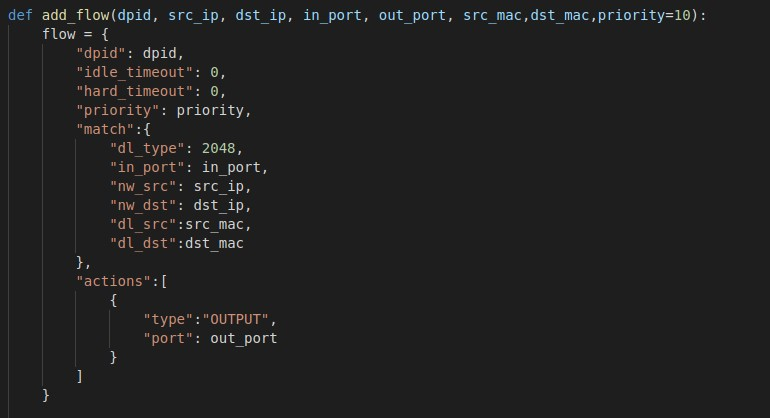
\includegraphics[width=0.7\linewidth]{19.jpg}
	\caption{下发流表代码}
\end{figure}
实际通信结果:\par
如图15是未匹配上二层匹配域的结果,这样不会产生环路,所以依然可以ping通。
\begin{figure}[H]
	\centering
	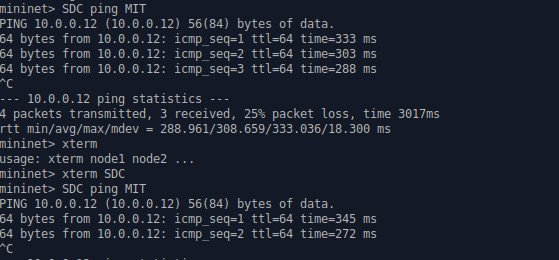
\includegraphics[width=0.9\linewidth]{21.jpg}
	\caption{未匹配上二层匹配域}
\end{figure}
下面查看SDC与MIT的二层地址,用于下发流表,将DL\_SRC = SDC\_MAC,DL\_DST = MIT\_MAC。
\begin{figure}[H]
	\centering
	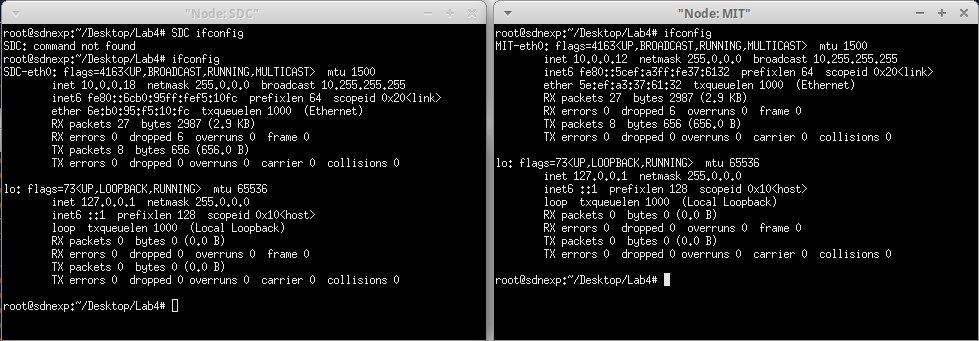
\includegraphics[width=0.9\linewidth]{22.jpg}
	\caption{查看SDC与MIT的网卡信息}
\end{figure}
如图15是匹配上二层匹配域的结果,这样会产生环路,所以不可以ping通。
\begin{figure}[H]
	\centering
	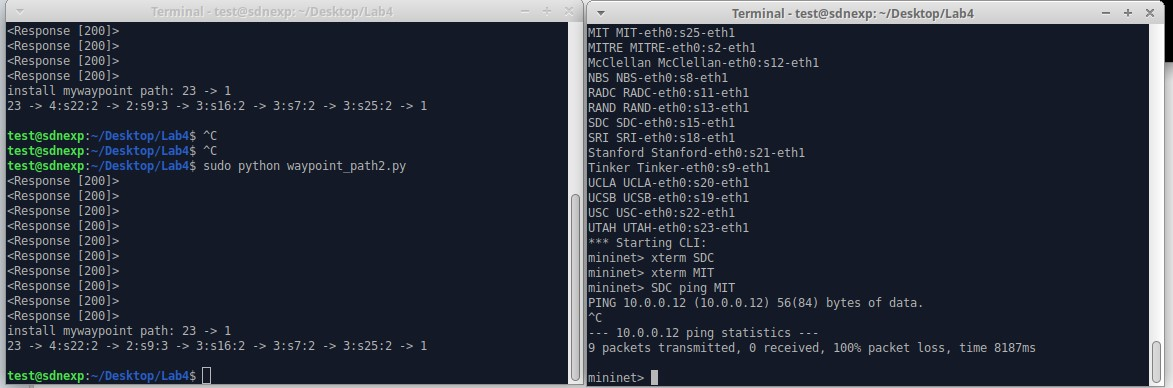
\includegraphics[width=0.9\linewidth]{23.jpg}
	\caption{匹配上二层匹配域}
\end{figure}
VeriFlow验证结果:\par
可以看出VeriFlow可以很好的验证出结果,考虑的匹配域比较全面。\par
\begin{figure}[H]
	\centering
	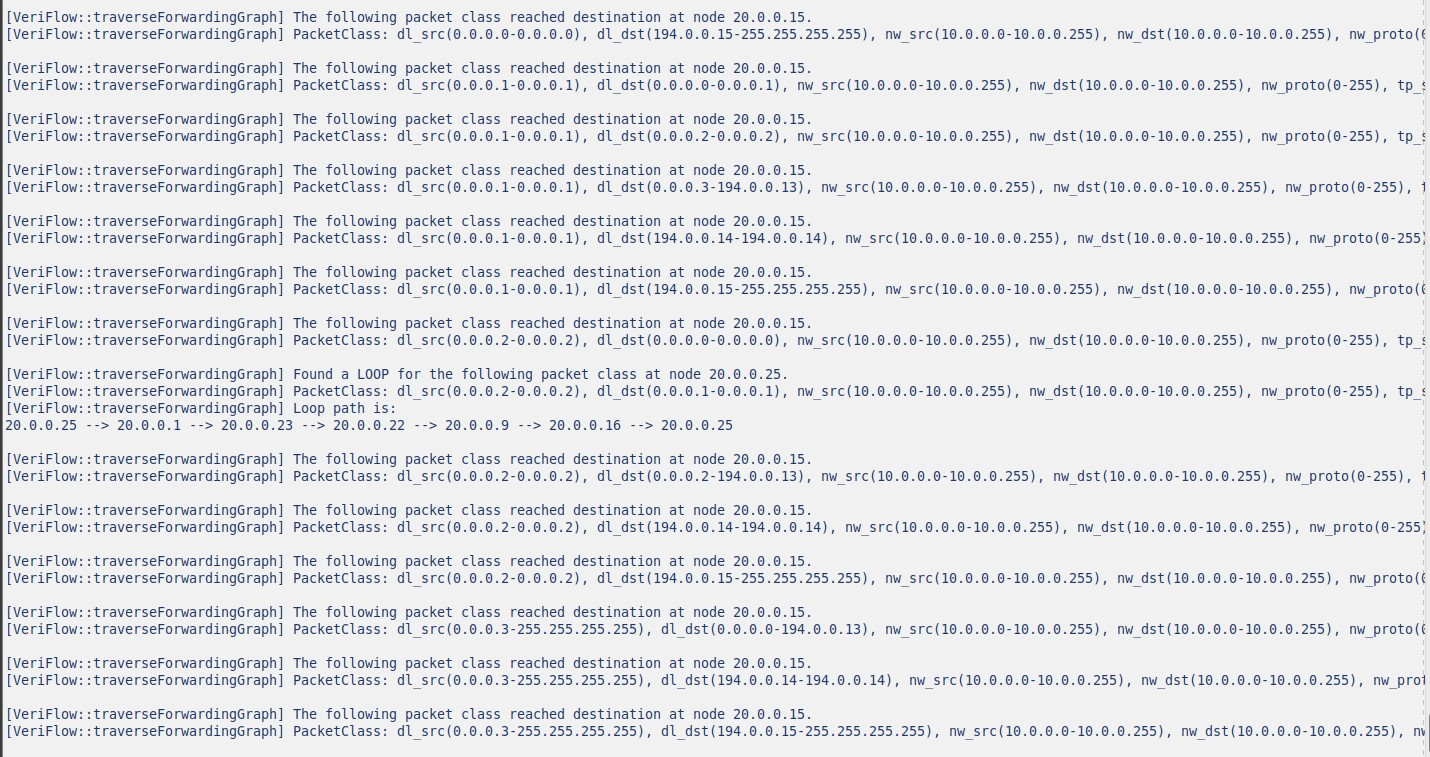
\includegraphics[width=0.9\linewidth]{20.jpg}
	\caption{流表验证}
\end{figure}
\subsubsection{挑选TCP/IP五元组进行验证}
在原下发列表的基础上,下发关于五元组的匹配元组,确定tp\_src=6666,tp\_dst=6666:
\begin{figure}[H]
	\centering
	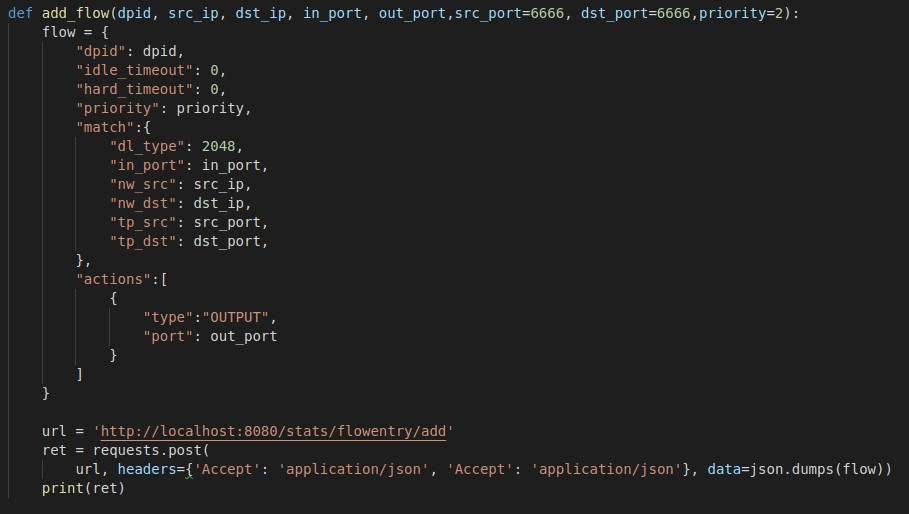
\includegraphics[width=0.7\linewidth]{15.jpg}
	\caption{下发流表代码}
\end{figure}
实际通信结果:\par
注意实验结果有BUG,因为Mininet的交换机只支持三层交换机,这里交换机不支持传输层流表,导致下发流表实际上还是三层流表与之前没有什么区别,导致切换成6667端口后仍然无法socket连接成功,理论上是应该成功的,与VeriFlow验证工具结果一致。
\begin{figure}[H]
	\centering
	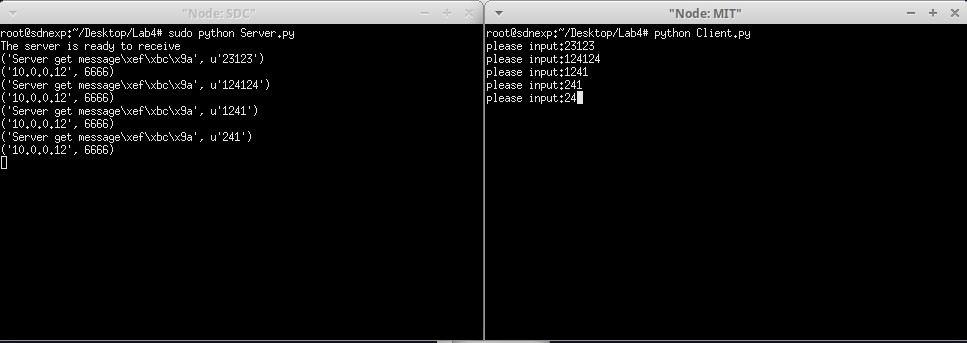
\includegraphics[width=0.9\linewidth]{16.jpg}
	\caption{下发流表前}
\end{figure}
\begin{figure}[H]
	\centering
	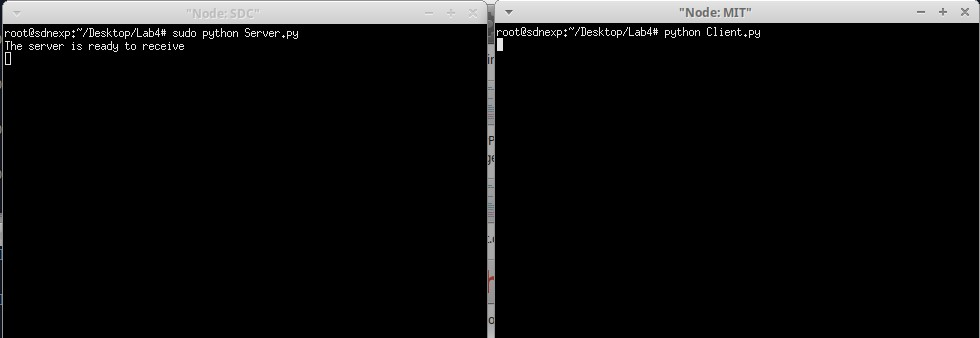
\includegraphics[width=0.9\linewidth]{17.jpg}
	\caption{下发流表后, socket绑定6666端口}
\end{figure}
\begin{figure}[H]
	\centering
	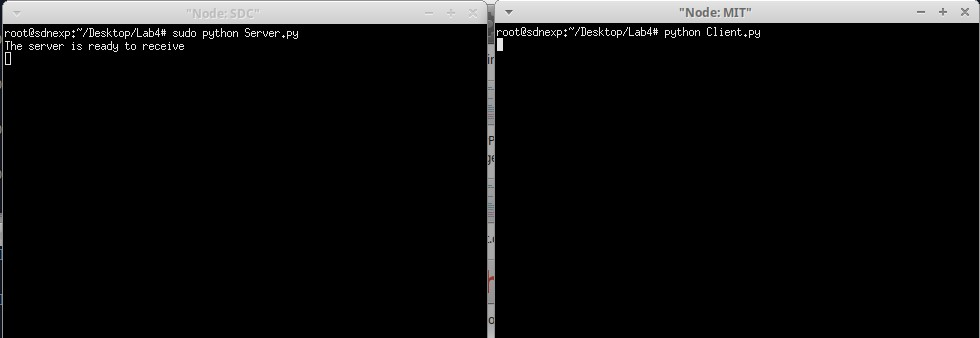
\includegraphics[width=0.9\linewidth]{17.jpg}
	\caption{下发流表后, socket绑定6667端口}
\end{figure}
VeriFlow验证结果:\par
可以看出与理论相符合。
\begin{figure}[H]
	\centering
	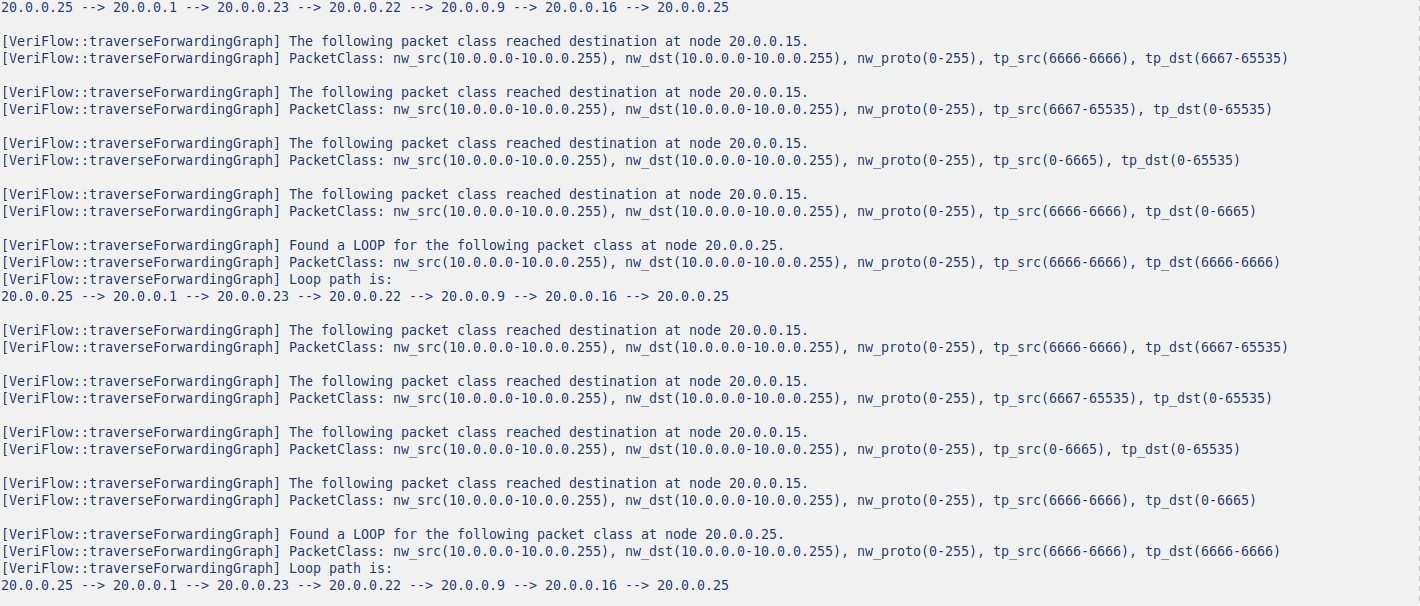
\includegraphics[width=0.9\linewidth]{18.jpg}
	\caption{流表验证}
\end{figure}
\subsubsection{多匹配域存在的问题}
在仔细实验操作后,就会发现实际上等价类划分与验证会与下发流表顺序有关系,例如在以上两个实验中,VeriFlow验证必须在先下发流表之后,再等SDCpingMIT的过程中,才会得到正确的等价类划分,正确全面分析网络。个人认为这里和Veriflow采用的数据结构trie树有关,词条树的匹配域顺序并不是固定的,导致划分的等价类不正确,一般必须先下发匹配域最多的流表,才能得到比较好的结果。虽然不全面的划分并不会导致错误的结果,但是全面的划分可以直观地显示网络通信状态,是更加合理的选择。
\begin{figure}[H]
	\centering
	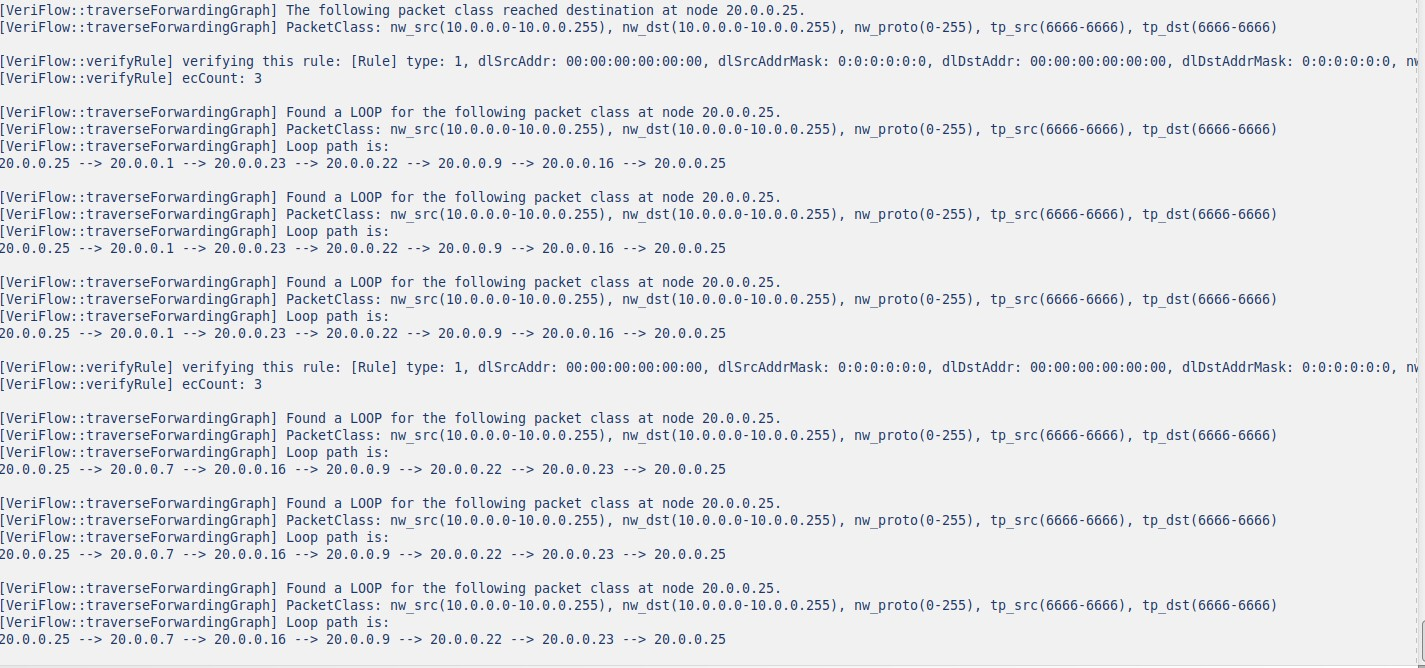
\includegraphics[width=0.9\linewidth]{24.jpg}
	\caption{顺序调换后不全面的等价类划分}
\end{figure}
\section{实验感悟}
1.对Veriflow的使用有了更深的理解,不再停留在理解层面,认识到了Veriflow的价值。\par 
2.在使用Veriflow的过程中,发现了许多该工具的bug和不全面性。\par 
3.由于时间原因,没有办法品读后人改进的论文,实属可惜,日后有时间再读。\par
\section{附录}
\subsection{下发二层匹配域流表}
\begin{lstlisting}[language=python]
import requests
import json

	def add_flow(dpid, src_ip, dst_ip, in_port, out_port, src_mac,dst_mac,priority=10):
		flow = {
			"dpid": dpid,
			"idle_timeout": 0,
			"hard_timeout": 0,
			"priority": priority,
			"match":{
				"dl_type": 2048,
				"in_port": in_port,
				"nw_src": src_ip,
				"nw_dst": dst_ip,
				"dl_src":src_mac,
				"dl_dst":dst_mac
			},
			"actions":[
			{
				"type":"OUTPUT",
				"port": out_port
			}
			]
		}

	url = 'http://localhost:8080/stats/flowentry/add'
	ret = requests.post(
	url, headers={'Accept': 'application/json'}, data=json.dumps(flow))
	print(ret)
	
	def show_path(src, dst, port_path):
		print('install mywaypoint path: {} -> {}'.format(src, dst))
		path = str(src) + ' -> '
		for node in port_path:
			path += '{}:s{}:{}'.format(*node) + ' -> '
			path += str(dst)
			path += '\n'
			print(path)

	def install_path():
		'23 -> 4:s22:2 -> 2:s9:3 -> 3:s16:2 -> 3:s7:2 -> 3:25:2 -> 1'
		src_sw, dst_sw = 23, 1
		waypoint_sw = 9  # Tinker 10.0.0.21, s9
		
		path = [(4, 22, 2), (2, 9, 3), (3, 16, 2), (3, 7, 2), (3, 25, 2)]
		# path = [(3, 7 , 2)]
		MIT_mac="6e:b0:95:f5:10:fc"
		SDC_mac="5e:ef:a3:37:61:32"
		# send flow mod
		for node in path:
		in_port, dpid, out_port = node
		add_flow(dpid, '10.0.0.0/24', '10.0.0.0/24', in_port, out_port,SDC_mac,MIT_mac)
		add_flow(dpid, '10.0.0.0/24', '10.0.0.0/24', out_port, in_port,MIT_mac,SDC_mac)
		show_path(src_sw, dst_sw, path)

if __name__ == '__main__':
	install_path()
\end{lstlisting}
\subsection{下发五元组流表}
\begin{lstlisting}[language=python]
import requests
import json

	def add_flow(dpid, src_ip, dst_ip, in_port, out_port,src_port=6666, dst_port=6666,priority=10):
		flow = {
			"dpid": dpid,
			"idle_timeout": 0,
			"hard_timeout": 0,
			"priority": priority,
			"match":{
				"dl_type": 2048,
				"in_port": in_port,
				"nw_src": src_ip,
				"nw_dst": dst_ip,
				"tp_src": src_port,
				"tp_dst": dst_port,
			},
			"actions":[
			{
				"type":"OUTPUT",
				"port": out_port
			}
			]
		}
	
		url = 'http://localhost:8080/stats/flowentry/add'
		ret = requests.post(
		url, headers={'Accept': 'application/json', 'Accept': 'application/json'}, data=json.dumps(flow))
		print(ret)

	def show_path(src, dst, port_path):
		print('install waypoint path: {} -> {}'.format(src, dst))
		path = str(src) + ' -> '
		for node in port_path:
		path += '{}:s{}:{}'.format(*node) + ' -> '
		path += str(dst)
		path += '\n'
		print(path)

	def install_path():
		'23 -> 4:s22:2 -> 2:s9:3 -> 3:s16:2 -> 3:s7:2 -> 3:25:2 -> 1'
		src_sw, dst_sw = 23, 1
		waypoint_sw = 9  # Tinker 10.0.0.21, s9
		
		path = [(4, 22, 2), (2, 9, 3), (3, 16, 2), (3, 7, 2), (3, 25, 2)] 
		# path = [(3, 7 , 2)]
		
		# send flow mod
		for node in path:
		in_port, dpid, out_port = node
		add_flow(dpid, '10.0.0.0/24', '10.0.0.0/24', in_port, out_port)
		add_flow(dpid, '10.0.0.0/24', '10.0.0.0/24', out_port, in_port)
		show_path(src_sw, dst_sw, path)

if __name__ == '__main__':
	install_path()	
\end{lstlisting}
\subsection{socket服务端与客户端}
\begin{lstlisting}[language=python]
#########Server.py
#coding:utf-8
import socket


	ip_port = ('10.0.0.18', 6666)
	back_log = 1
	serverSocket = socket.socket(socket.AF_INET, socket.SOCK_STREAM)
	serverSocket.setsockopt(socket.SOL_SOCKET, socket.SO_REUSEADDR, 1)
	serverSocket.bind(ip_port) 
	serverSocket.listen(back_log)
	print('The server is ready to receive')
	connectionSocket, addr = serverSocket.accept()
	while 1:
		msg = connectionSocket.recv(1024).decode()  
		if msg == '1':
			connectionSocket.close()
			break
		print("Server get message:",msg)
		print(addr)                                
	serverSocket.close()
#########Client.py	
#coding:utf-8
import socket


	clientSocket = socket.socket(socket.AF_INET, socket.SOCK_STREAM)
	clientSocket.bind(('10.0.0.12', 6667))
	clientSocket.connect(('10.0.0.18', 6666))
	while 1:
		msg = str(raw_input('please input:'))
		if not msg:
			continue
		clientSocket.sendall(msg.encode())
		if msg == '1':
			break
	clientSocket.close()
\end{lstlisting}
\end{document}
